
\section{Integración de GRASS}\label{sec:grass}\index{GRASS}

El complemento de GRASS~\cite{GRASSweb} proporciona acceso a GRASS desde dentro de QGIS. Esto incluye la capacidad de ver, editar y crear datos, así como realizar análisis usando los módulos de geoprocesamiento de GRASS.

En este capítulo presentaremos el complemento y alguna de las formas que se pueden usar para trabajar con datos de GRASS. El complemento de GRASS proporciona las siguientes funciones:
 
\begin{itemize}
\item 
\includegraphics[width=0.7cm]{add_grass_vector} Añadir capas vectoriales de GRASS.
\item 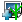
\includegraphics[width=0.7cm]{add_grass_raster} Añadir capas ráster de GRASS.
\item 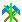
\includegraphics[width=0.7cm]{grass_tools} Caja de herramientas de GRASS.
\item 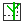
\includegraphics[width=0.7cm]{grass_region_edit} Cambiar la región de GRASS.
\item 
\includegraphics[width=0.7cm]{grass_edit} Digitalización de capas vectoriales.
\item 
\includegraphics[width=0.7cm]{grass_open_mapset} Abrir directorios de mapas existentes.
\item 
\includegraphics[width=0.7cm]{grass_new_mapset} Crear nuevos directorios de mapas.
\item 
\includegraphics[width=0.7cm]{grass_new_vector_layer} Crear nuevas capas vectoriales de GRASS.
\item 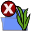
\includegraphics[width=0.7cm]{grass_close_mapset} Cerrar directorios de mapas de GRASS.
\end{itemize}

\subsection{Iniciar QGIS con GRASS}\label{sec:starting_grass}
\index{GRASS!starting QGIS}

Para usar las funciones de GRASS desde dentro de QGIS, debe cargar el complemento de GRASS con el administrador de complementos (vea la Sección \ref{sec:managing_plugins}) como todos los complementos de QGIS. Después de cargarlo, aparecerá una nueva barra de herramientas en la interfaz de usuario.\footnote{El complemento de GRASS es único en cuanto que crea su propia barra de herramientas}

Después de cargar el complemento, inmediatamente puede cargar un conjunto de datos vectoriales y ráster de GRASS existente (vea la Sección \ref{sec:load_grassdata}) o puede crear una nueva localización de GRASS con QGIS (vea la Sección \ref{sec:create_loc}).

\subsection{Cargar datos de GRASS}\label{sec:load_grassdata}\index{GRASS!loading data}

Con el complemento de GRASS, puede cargar capas vectoriales o ráster usando los botones adecuados de la barra de herramientas. Como ejemplo usaremos la localización spearfish de muestra en proyección UTM (vea la Sección \ref{label_sampledata}).

\begin{enumerate}
  \item Descargue el archivo spearfish\_grass60data-0.3.zip.
  \item Cree una carpeta nueva \textsl{grassdata} y descomprima en ella el archivo spearfish\_grass60data-0.3.zip.
  \item Inicie QGIS.
  \item En la barra de herramientas de GRASS, pulse el icono \textsl{Abrir directorio de mapas} para iniciar el asistente \textsl{Seleccionar directorio de mapas de GRASS}.
  \item Para la \textsl{Base de datos} explore e introduzca la ruta a la carpeta recién creada \textsl{grassdata}.
  \item Ahora debería poder seleccionar la localización \textsl{spearfish60} y los directorios de mapas \textsl{PERMANENT} o \textsl{user1}. 
  \item Pulse \textsl{Aceptar}. Note como algunas de las herramientas de la barra de herramientas de GRASS que estaban desactivadas ahora están activadas.
  \item Pulse en \textsl{Añadir capa ráster de GRASS}, seleccione el \textsl{Nombre del mapa} geology y pulse \textsl{Aceptar}. El mapa geology se visualizará. 
  \item Pulse en \textsl{Añadir capa vectorial de GRASS}, seleccione el \textsl{Nombre del mapa} roads (carreteras) y pulse \textsl{Aceptar}. Ahora el mapa roads se superpondrá encima de la geología.  
\end{enumerate}

Como puede ver, es muy sencillo cargar capas ráster y vectoriales de GRASS en QGIS. Vea las siguientes secciones para editar datos de GRASS y crear nuevas localizaciones.

\begin{Tip}\caption{\textsc{Cargar datos de GRASS}}
\qgistip{Si tiene problemas para cargar datos o QGIS termina de forma anormal, asegúrese de que ha cargado el complemento de GRASS correctamente como se describe en la Sección \ref{sec:starting_grass}.
}
\end{Tip} 

\subsection{Crear una localización}\label{sec:create_loc}

GRASS guarda los datos en una ``localización'' que representa un área específica con un sistema de coordenadas específico. Para usar datos de GRASS, debemos importarlos a una \textsl{localización}.\footnote{Esto no es estrictamente cierto, se pueden ver conjuntos de datos externos sin importarlos}

\begin{figure}[ht]
   \begin{center}
   \caption{Crear una localización de GRASS en QGIS}\label{fig:grass_location}\smallskip
   
\includegraphics[clip=true, width=8cm]{grass_location}
\end{center}  
\end{figure}

Aquí tiene un ejemplo de cómo crear una localización de GRASS en la proyección Albers Equal Area con unidades en metros para los datos de ejemplo de QGIS (vea la Sección \ref{label_sampledata}). 

\begin{enumerate}
  \item Inicie QGIS.
  \item Asegúrese de que el complemento de GRASS está cargado.
  \item Cargue el archivo shape \textsl{alaska.shp} (vea la Sección \ref{sec:load_shapefile}).
  \item En la barra de herramientas de GRASS, pulse en la herramienta \textsl{Nuevo directorio de mapas} para llamar al asistente directorio de mapas.
  \item Cada localización se guarda en un directorio. Seleccione un directorio de datos existente o cree uno nuevo para guardar la localización.
  \item Pulse \textsl{Siguiente}.
  \item Podemos usar el asistente para crear un nuevo directorio de mapas dentro de una localización existente o crear una nueva localización todo junto. Marque el botón circular ``Crear nueva localización''.
  \item Introduzca un nombre para la localización (usaremos Alaska).
  \item Pulse \textsl{Siguiente}.
  \item Defina la proyección pulsando el botón circular ``Proyección'' para activar la lista de proyecciones.
  \item Estamos usando la proyección Albers Equal Area Alaska (metros). Como sabemos que su SRID de PostGIS es 5000, lo introducimos en la casilla de búsqueda. (Si quiere repetir este proceso para otra capa y no recuerda el SRID de PostGIS, pulse en el icono del proyector en la esquina inferior derecha de la barra de estado (vea la Sección \ref{label_projstart}).)
  \item Pulse \textsl{Encontrar} para seleccionar la proyección.
  \item Pulse \textsl{Siguiente}.
  \item Para definir la región predeterminada, tenemos que introducir los límites en dirección Norte, Sur, Este y Oeste. Aquí simplemente pulsaremos el botón \textsl{Establecer la extensión actual de QGIS}.
  \item Pulse \textsl{Siguiente}. 
  \item Tenemos que definir un directorio de mapas dentro de nuestra nueva localización. Póngale el nombre que prefiera (su nombre de usuario es una buena opción).
  \item Compruebe el resumen para asegurarse que es correcto.
  \item Pulse \textsl{Terminar} 
  \item El directorio de mapas y la localización son creados y se abren como el conjunto de trabajo actual.
  \item Vea como algunas de las herramientas de la barra de herramientas de GRASS que estaban desactivadas ahora están activadas para su uso.
\end{enumerate}

Si le parecieron muchos pasos, ésto no es tan malo y sí una forma muy rápida de crear una localización. Nuestra localización ahora está lista para usar. Para ver la región predeterminada, aleje el zum. Pulsando la herramienta \textsl{Mostrar región actual de Grass} se activa/desactiva la visualización de la región.

\subsection{Modelo de datos vectoriales}\label{label_vectmodel}\index{GRASS!vector data model}

Es importante entender el modelo de datos vectoriales de GRASS antes de digitalizar.\index{GRASS!digitizing} En general, GRASS usa un modelo vectorial topológico.\index{GRASS!topology} Esto significa que las áreas no se representan como polígonos cerrados, sino por uno o más contornos. Esto significa que las áreas no se representan como polígonos cerrados, sino por uno o más contornos. Los contornos deben estar conectados sin saltos. Un área es identificada (etiquetada) por los centroides del área.

Además de contornos y centroides, un mapa vectorial puede contener puntos y líneas. Todos estos elementos geométricos pueden mezclarse en un vectorial y se representarán en las llamadas «capas» en QGIS.

Es posible guardar más «capas» en un conjunto de datos vectorial. Por ejemplo, se pueden guardar campos, bosques y lagos en un vectorial. Los bosques y lagos adyacentes pueden compartir el mismo contorno, pero tiene tablas de atributos separadas. También es posible adjuntar atributos a los contornos. Por ejemplo, el contorno entre lago y bosque es una carretera, por lo que puede tener una tabla de atributos diferente.

La «capa» de los objetos espaciales se define por la «capa» dentro de GRASS. «Capa» es un número que define si hay más de una capa dentro del conjunto de datos, por ejemplo, si la geometría es bosque o lago. De momento, puede ser sólo un número, en el futuro GRASS también soportará nombre como campos en la interfaz de usuario.

Los atributos se pueden guardar en bases de datos externas, por ejemplo DBF, PostgreSQL, MySQL, SQLite3, etc.\index{GRASS!attribute storage}

Los atributos en las tablas de las bases de datos se enlazan a los elementos geométricos usando la «categoría».\index{GRASS!attribute linkage} La «categoría» (clave, ID) es un entero adjunto a los primitivos de la geometría y se usa como el enlace a una columna de la tabla de la base de datos.

\begin{Tip}\caption{\textsc{Aprender el modelo vectorial de GRASS}}
\qgistip{La mejor forma de aprender el modelo vectorial de GRASS y sus capacidades es descargar uno de los muchos manuales de GRASS, donde se describe el modelo vectorial con más detalle. Vea \url{http://grass.osgeo.org/gdp/manuals.php} para más información, libros y manuales en varios idiomas.
}
\end{Tip} 

\subsection{Herramientas de digitalización y edición}\index{GRASS!digitizing tools}
\label{grass_digitising}


\includegraphics[width=0.7cm]{grass_edit} Las herramientas de digitalización para las capas vectoriales de GRASS son accesibles usando la herramienta \textsl{Editar capa vectorial de GRASS} de la barra de herramientas. Asegúrese de que ha cargado un vectorial de GRASS y que éste es la capa seleccionada en la leyenda antes de pulsar la herramienta de edición. Si quiere crear un nuevo vectorial de GRASS, necesita usar la entrada de menú Complementos->GRASS->Crear nuevo vectorial de GRASS o el icono de la barra de herramientas de Grass.

La figura \ref{fig:grass_edit} muestra el diálogo de edición de GRASS que se muestra cuando se pulsa la herramienta de edición.

\begin{figure}[h]
   \begin{center}
   \caption{Diálogo de edición de GRASS}\label{fig:grass_edit}\smallskip
   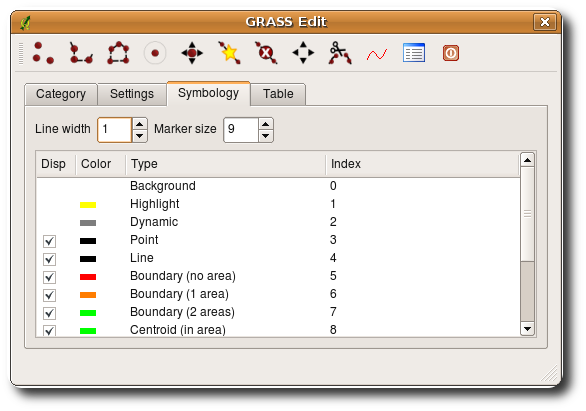
\includegraphics[clip=true, width=13cm]{grassedit}
\end{center}  
\end{figure}

Las herramientas y la configuración se tratan en las siguientes secciones.

\subsubsection{Barra de herramientas}\label{label_grasstoolbar}

La tabla \ref{tab:grass_tools} lista las herramientas de digitalización proporcionadas por el complemento de GRASS. Éstas corresponden a los botones de herramientas en la barra de herramientas de la parte superior del diálogo.

\begin{table}[h]\index{GRASS!digitizing tools}
\centering
\caption{Herramientas de digitalización de GRASS}\label{tab:grass_tools}\medskip
 \begin{tabular}{|l|l|p{5in}|}
 \hline \textbf{Icono} & \textbf{Herramienta} & \textbf{Propósito} \\
\hline 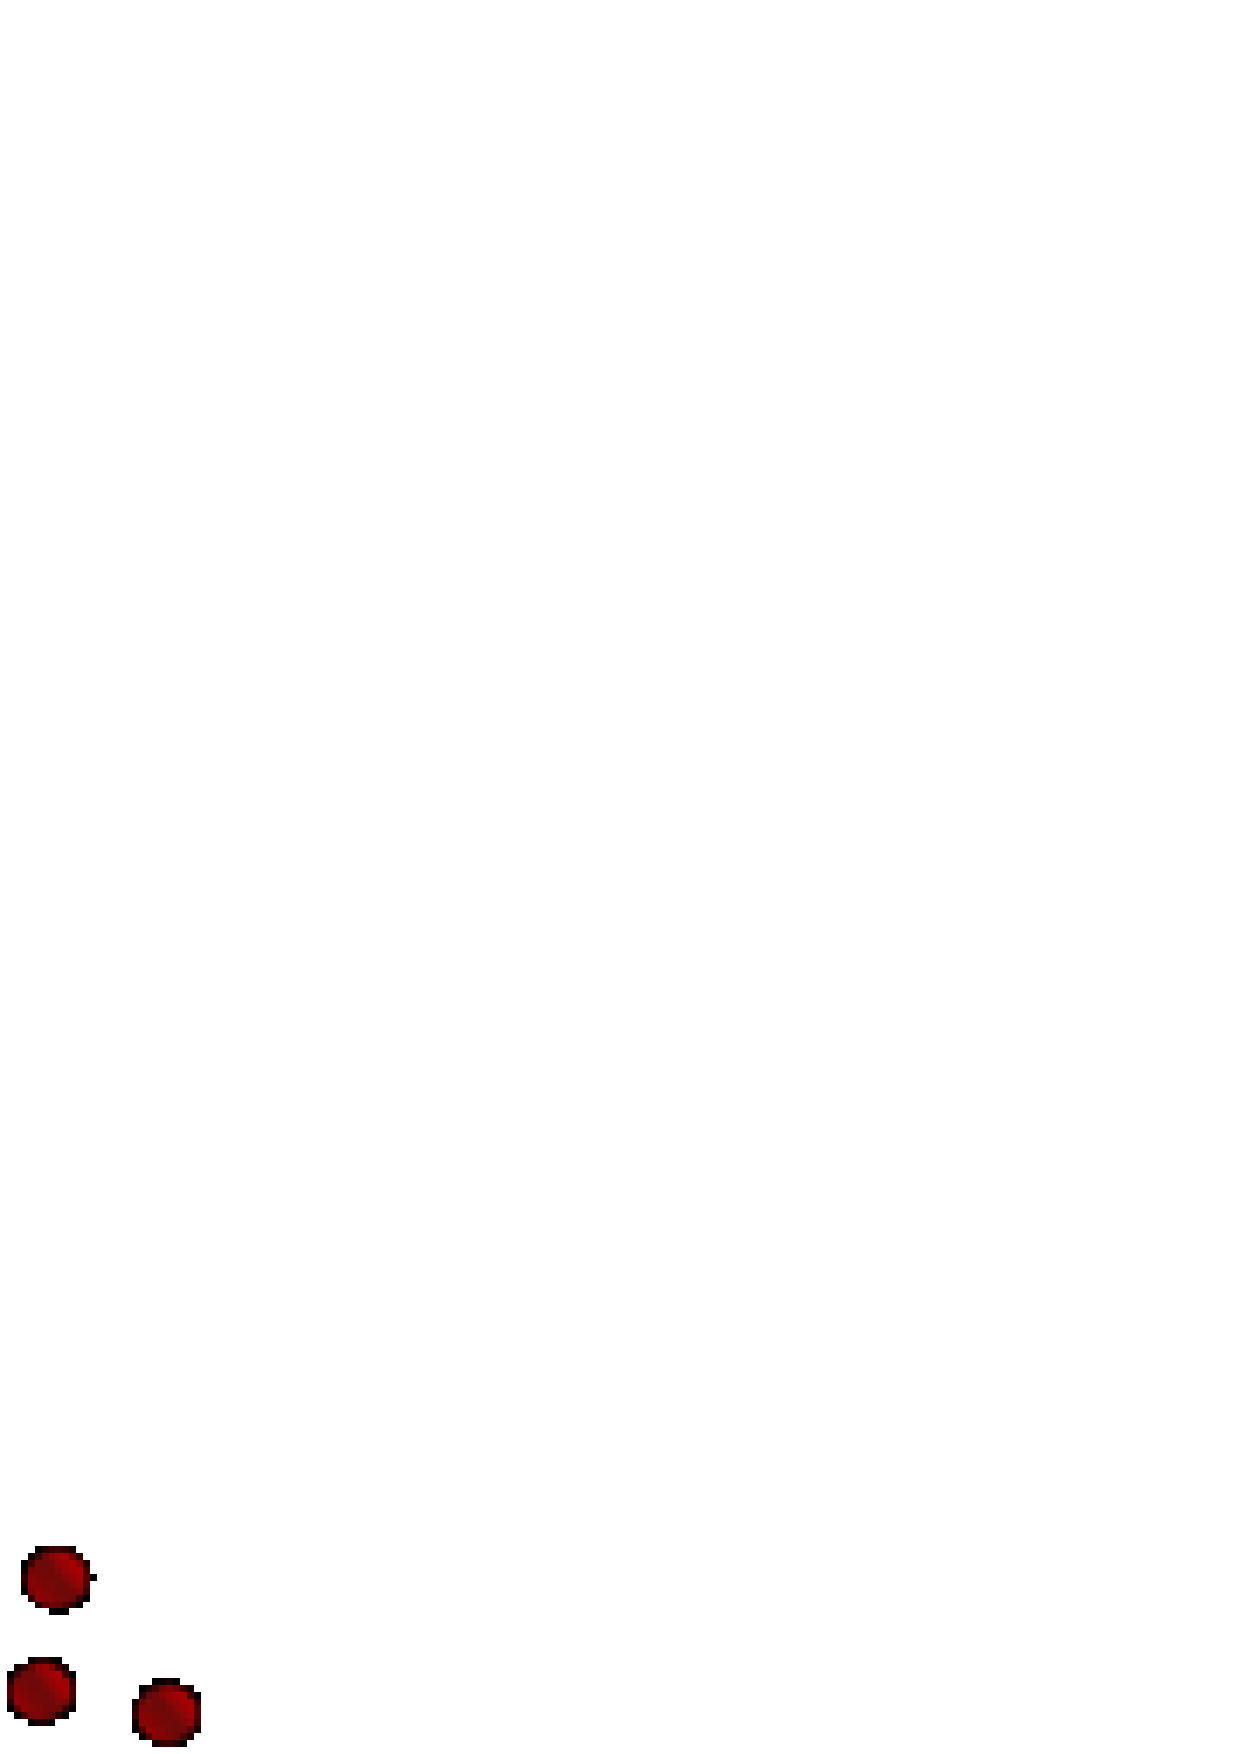
\includegraphics[width=0.7cm]{grass_new_point} & Nuevo punto & Digitalizar un punto nuevo \\
\hline 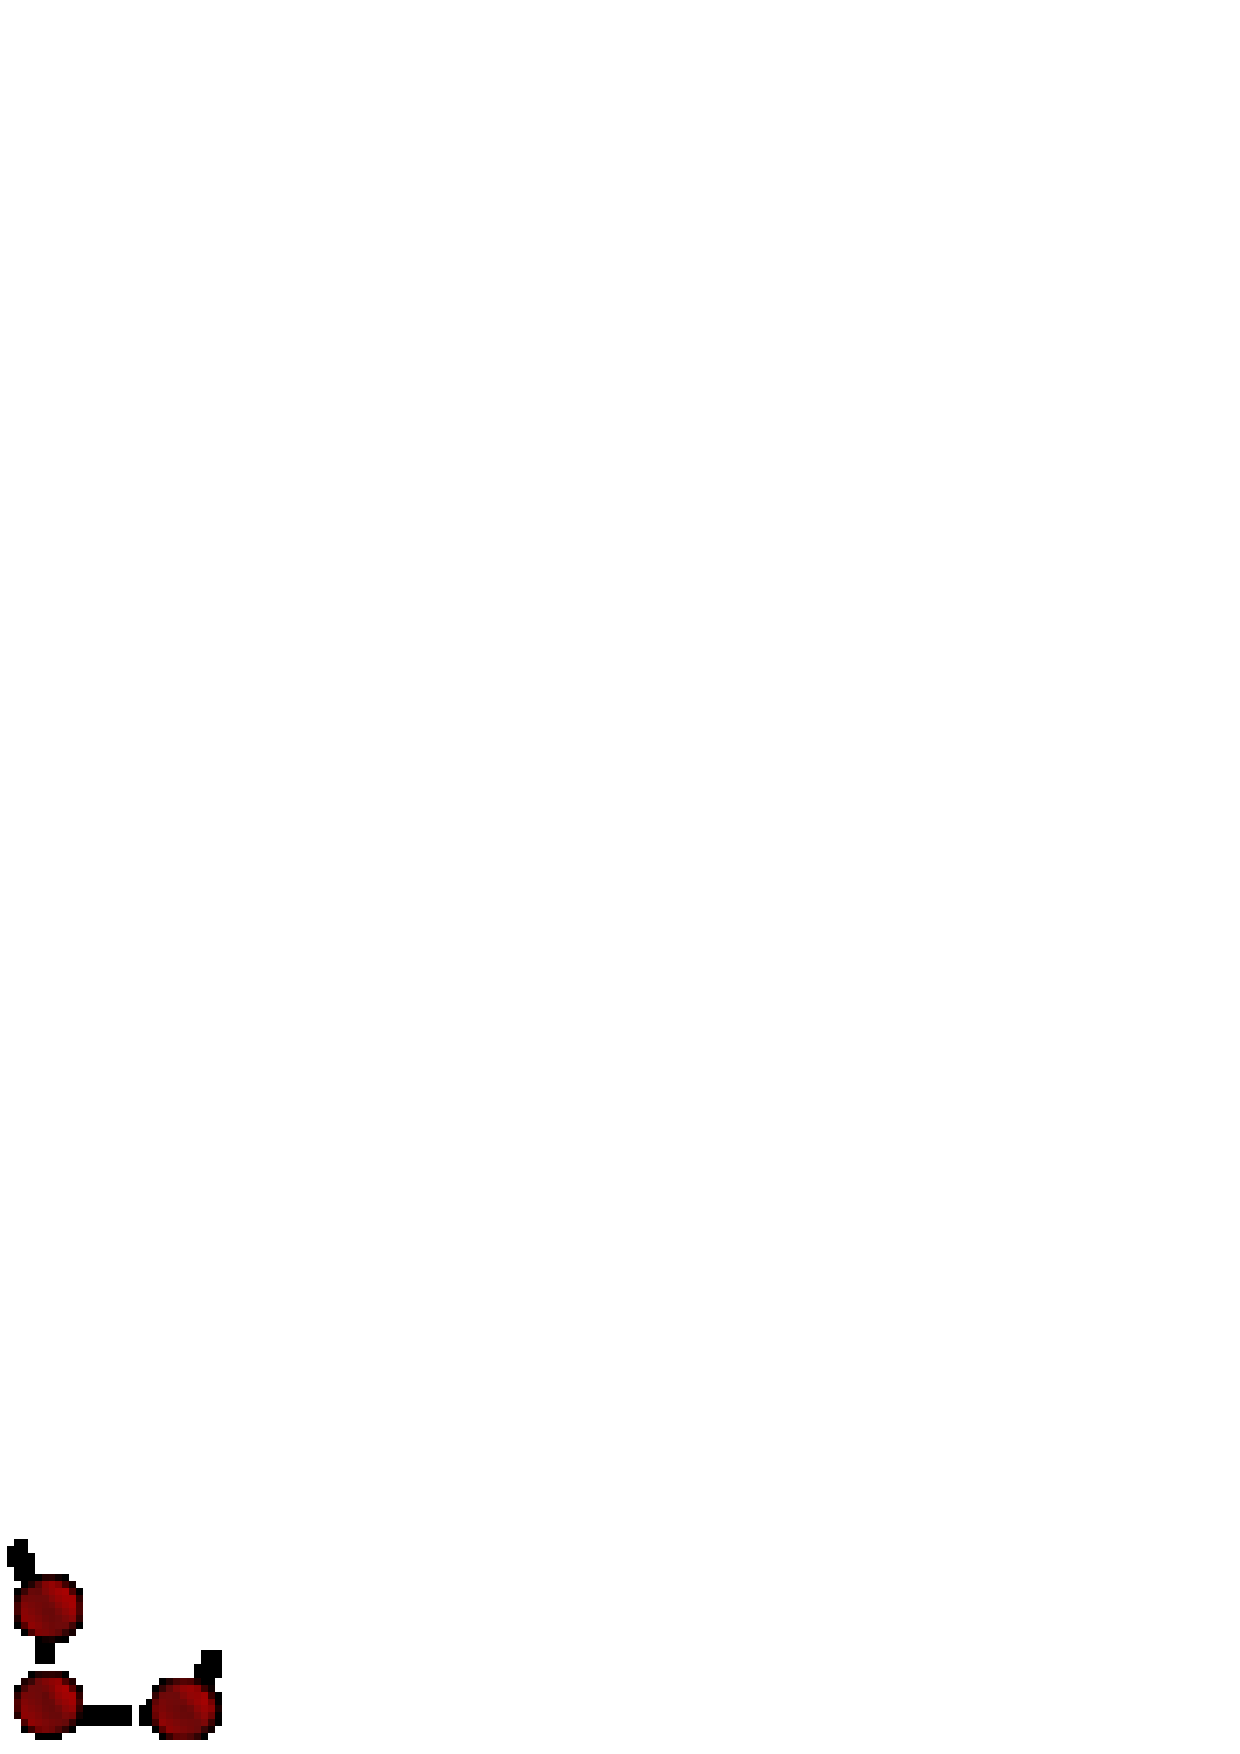
\includegraphics[width=0.7cm]{grass_new_line} & Nueva línea &  Digitalizar una línea nueva (finaliza al seleccionar una herramienta nueva) \\
\hline 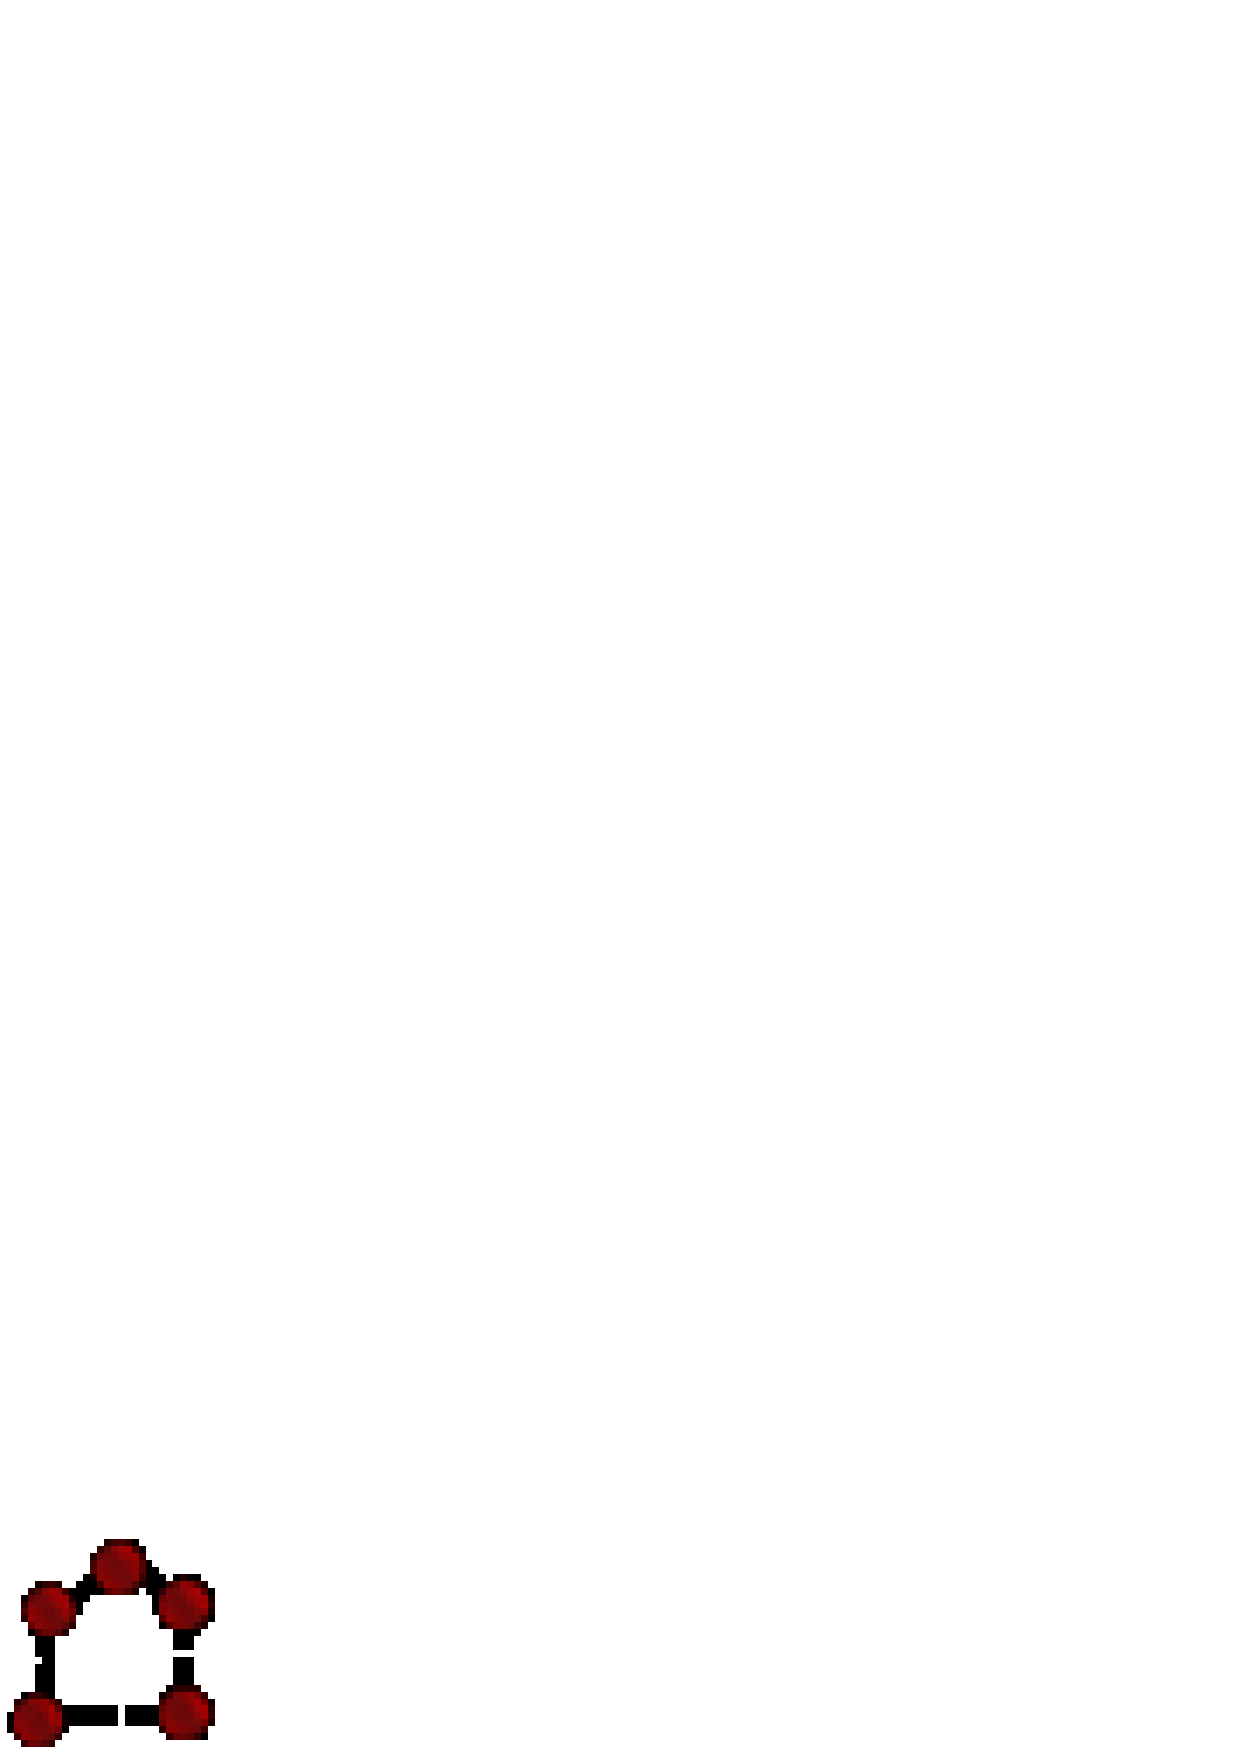
\includegraphics[width=0.7cm]{grass_new_boundary} & Nuevo contorno & Digitalizar un contorno nuevo (finaliza al seleccionar una herramienta nueva)\\
\hline 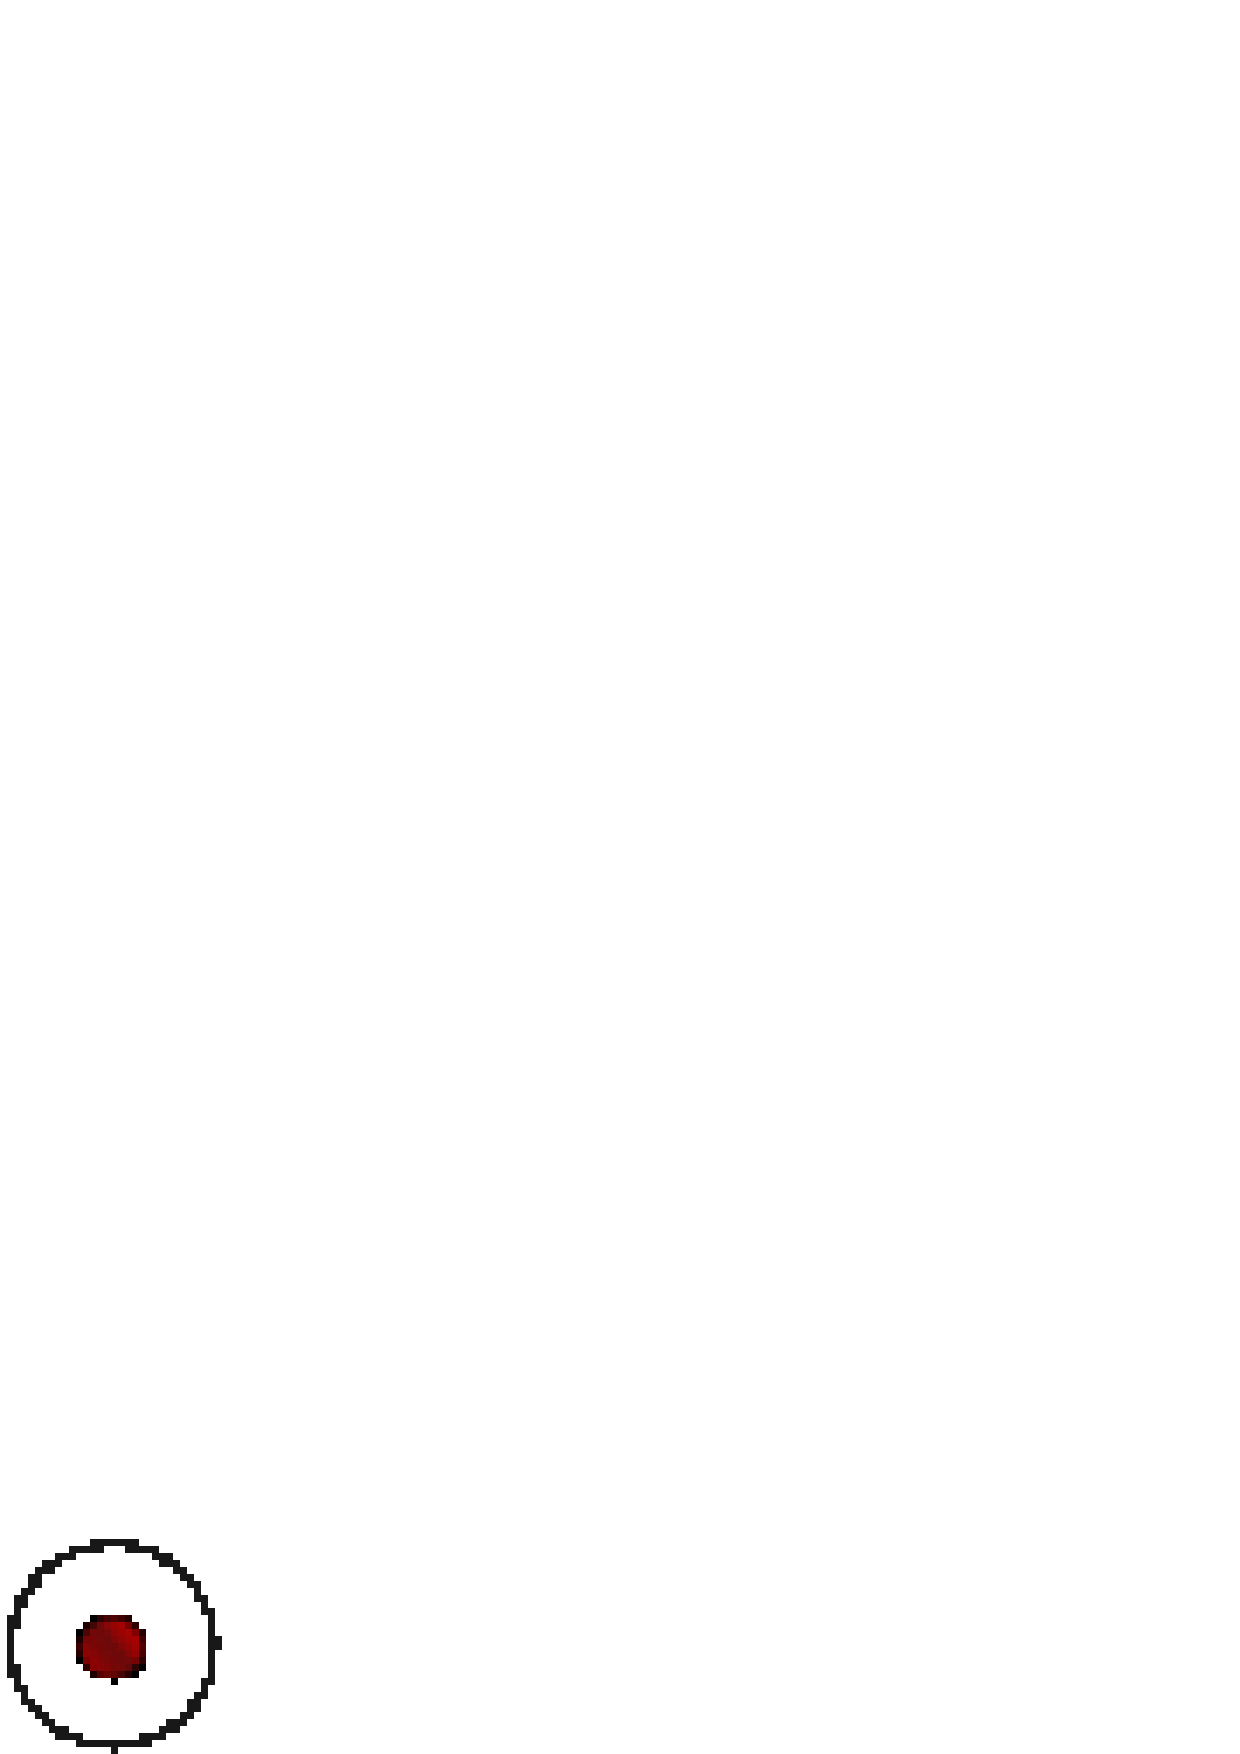
\includegraphics[width=0.7cm]{grass_new_centroid} & Nuevo centroide & Digitalizar un centroide nuevo (etiquetar un área existente)\\
\hline 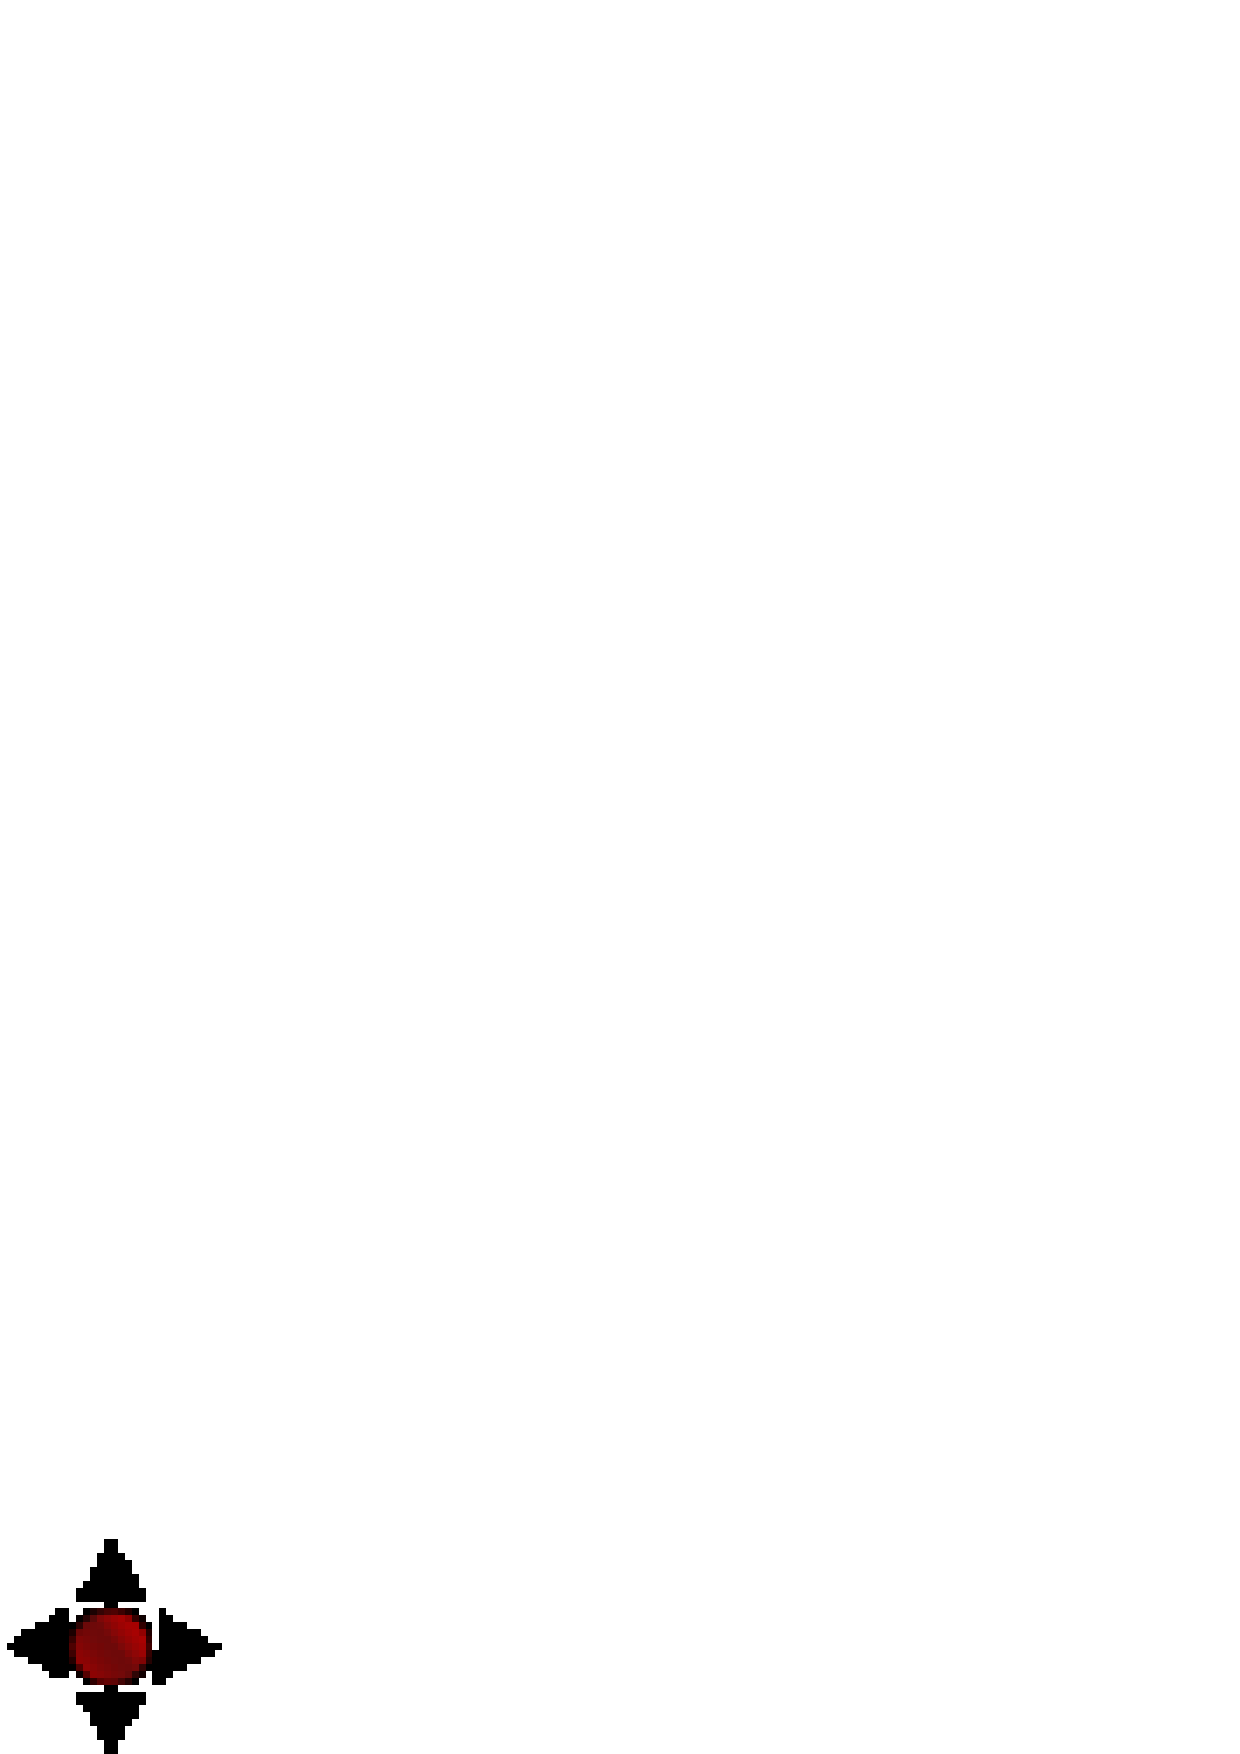
\includegraphics[width=0.7cm]{grass_move_vertex} & Mover vértice & Seleccionar un vértice de una línea o contorno existente e identificar una nueva posición\\
\hline 
\includegraphics[width=0.7cm]{grass_add_vertex} & Añadir vértice & Añadir un vértice nuevo a una línea existente\\
\hline 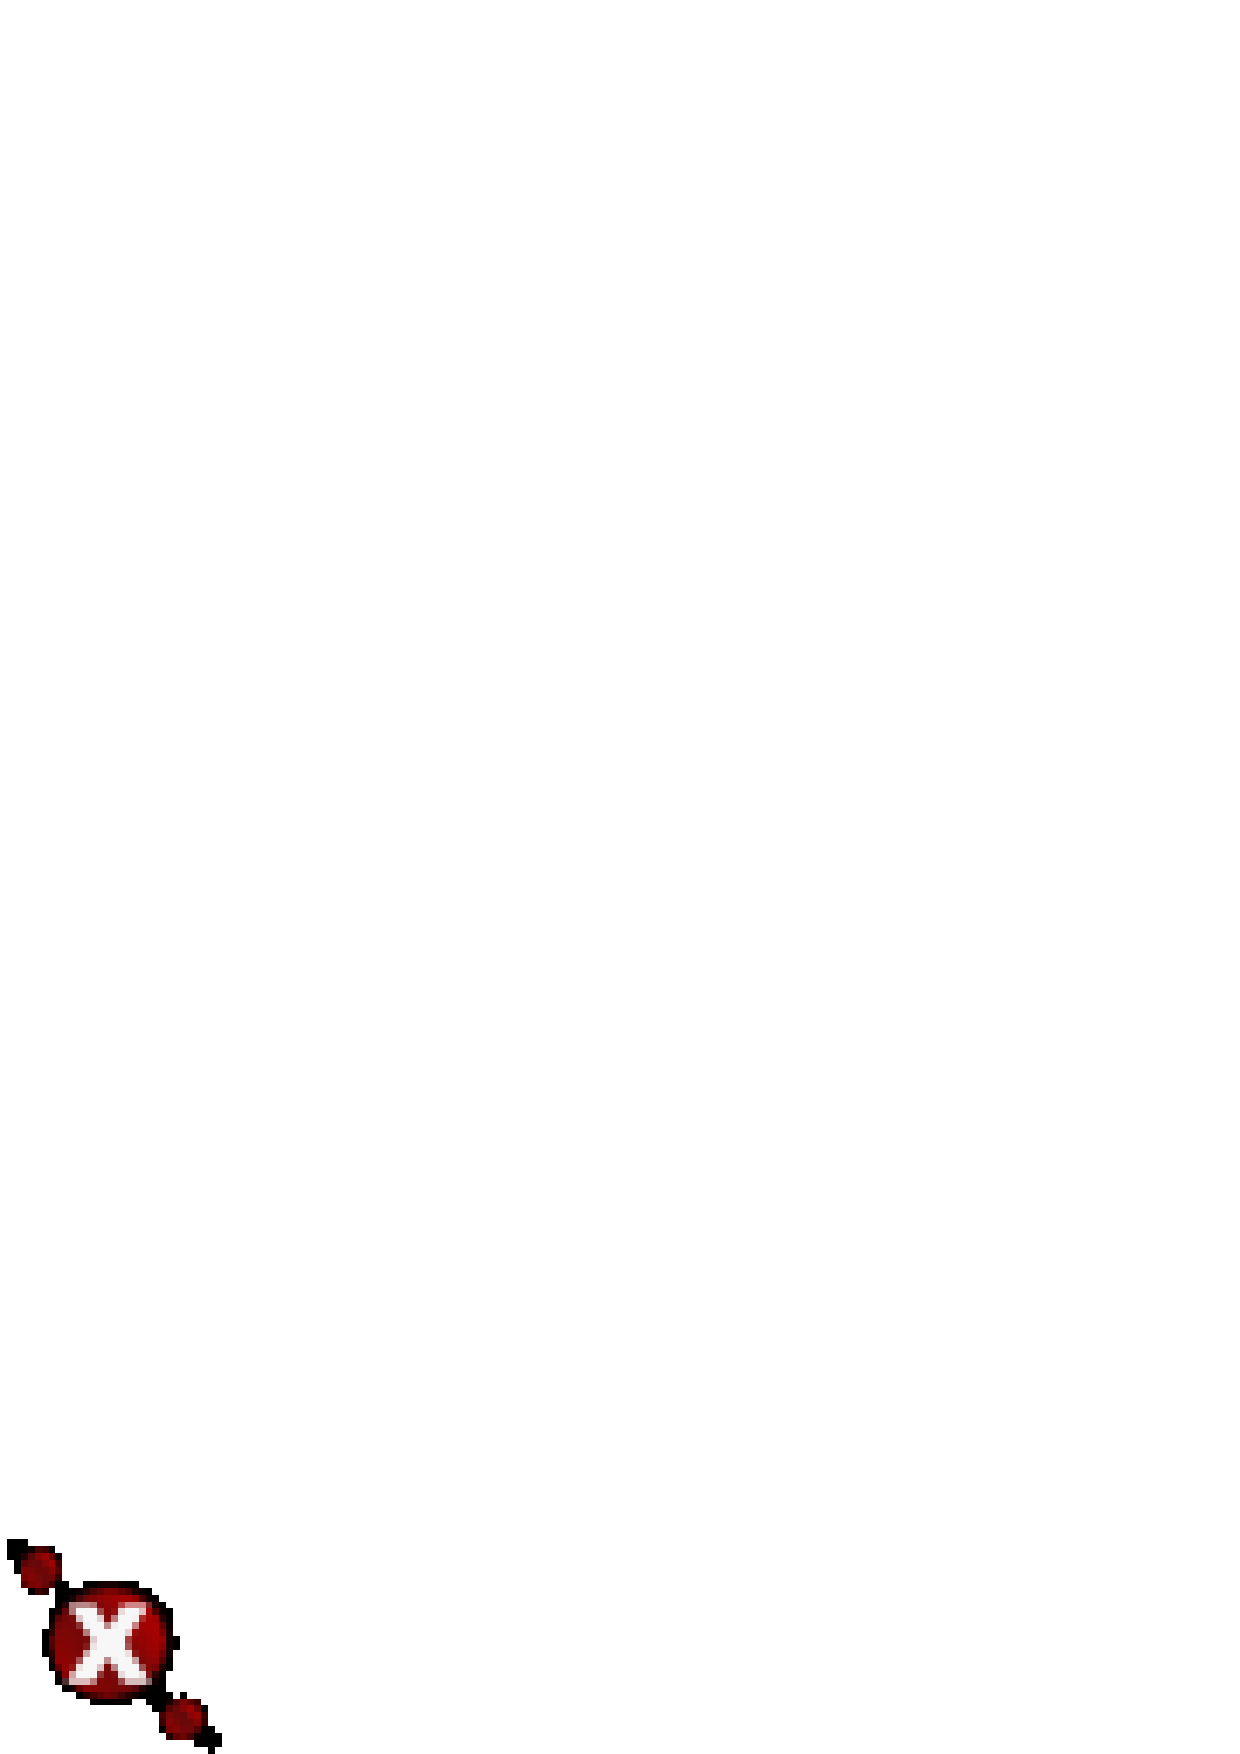
\includegraphics[width=0.7cm]{grass_delete_vertex} & Borrar vértice & Borrar un vértice de una línea existente (confirmar el vértice seleccionado con otra pulsación)\\
\hline 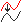
\includegraphics[width=0.7cm]{grass_move_line} & Mover elemento & Seleccionar un elemento existente y pulsar en la nueva posición\\
\hline 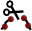
\includegraphics[width=0.7cm]{grass_split_line} & Dividir línea & Dividir una línea existente en dos partes\\
\hline 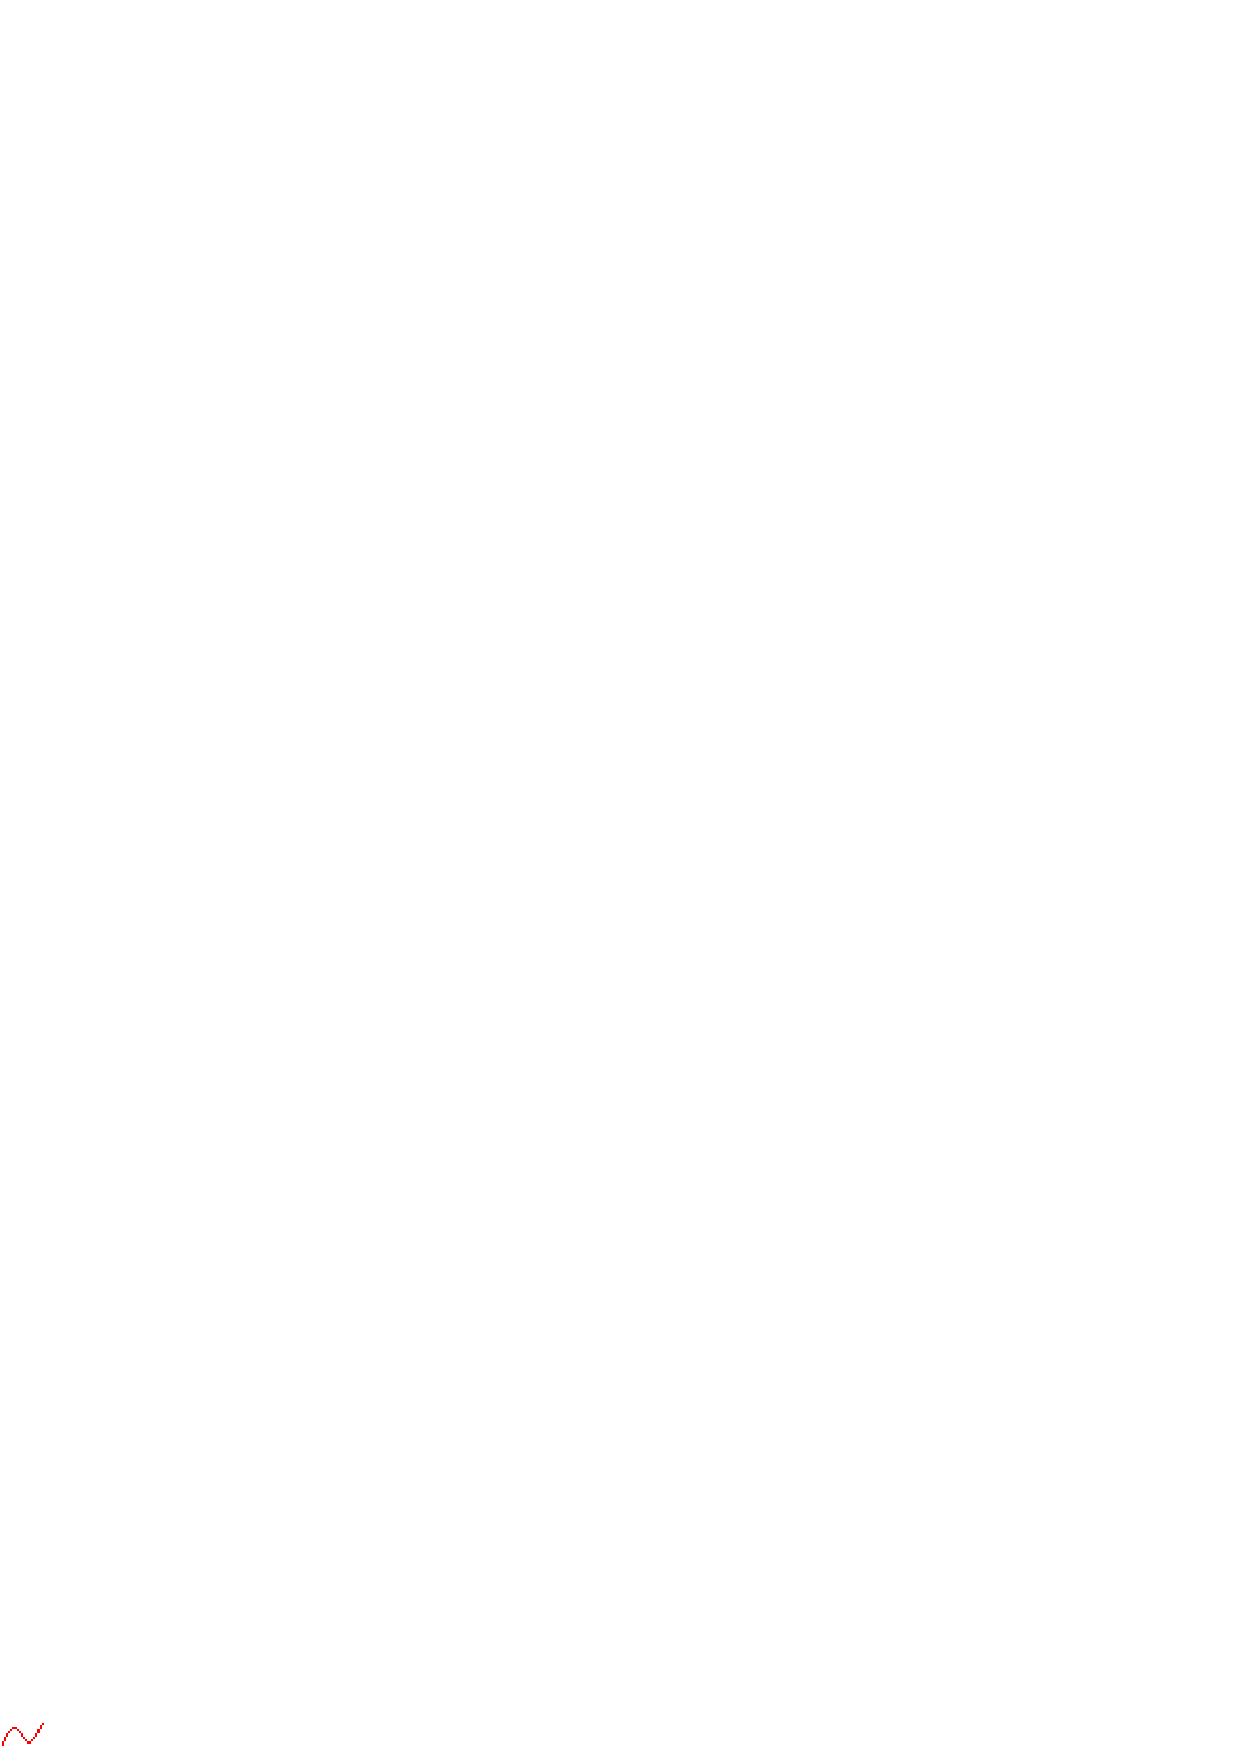
\includegraphics[width=0.7cm]{grass_delete_line} & Borrar elemento & Borrar un elemento existente (confirmar el elemento seleccionado con otra pulsación)\\
\hline 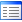
\includegraphics[width=0.7cm]{grass_edit_attributes} & Editar atributos & Editar los atributos de un elemento existente (tenga en cuenta que un elemento puede representar a más objetos espaciales, vea arriba)\\
\hline 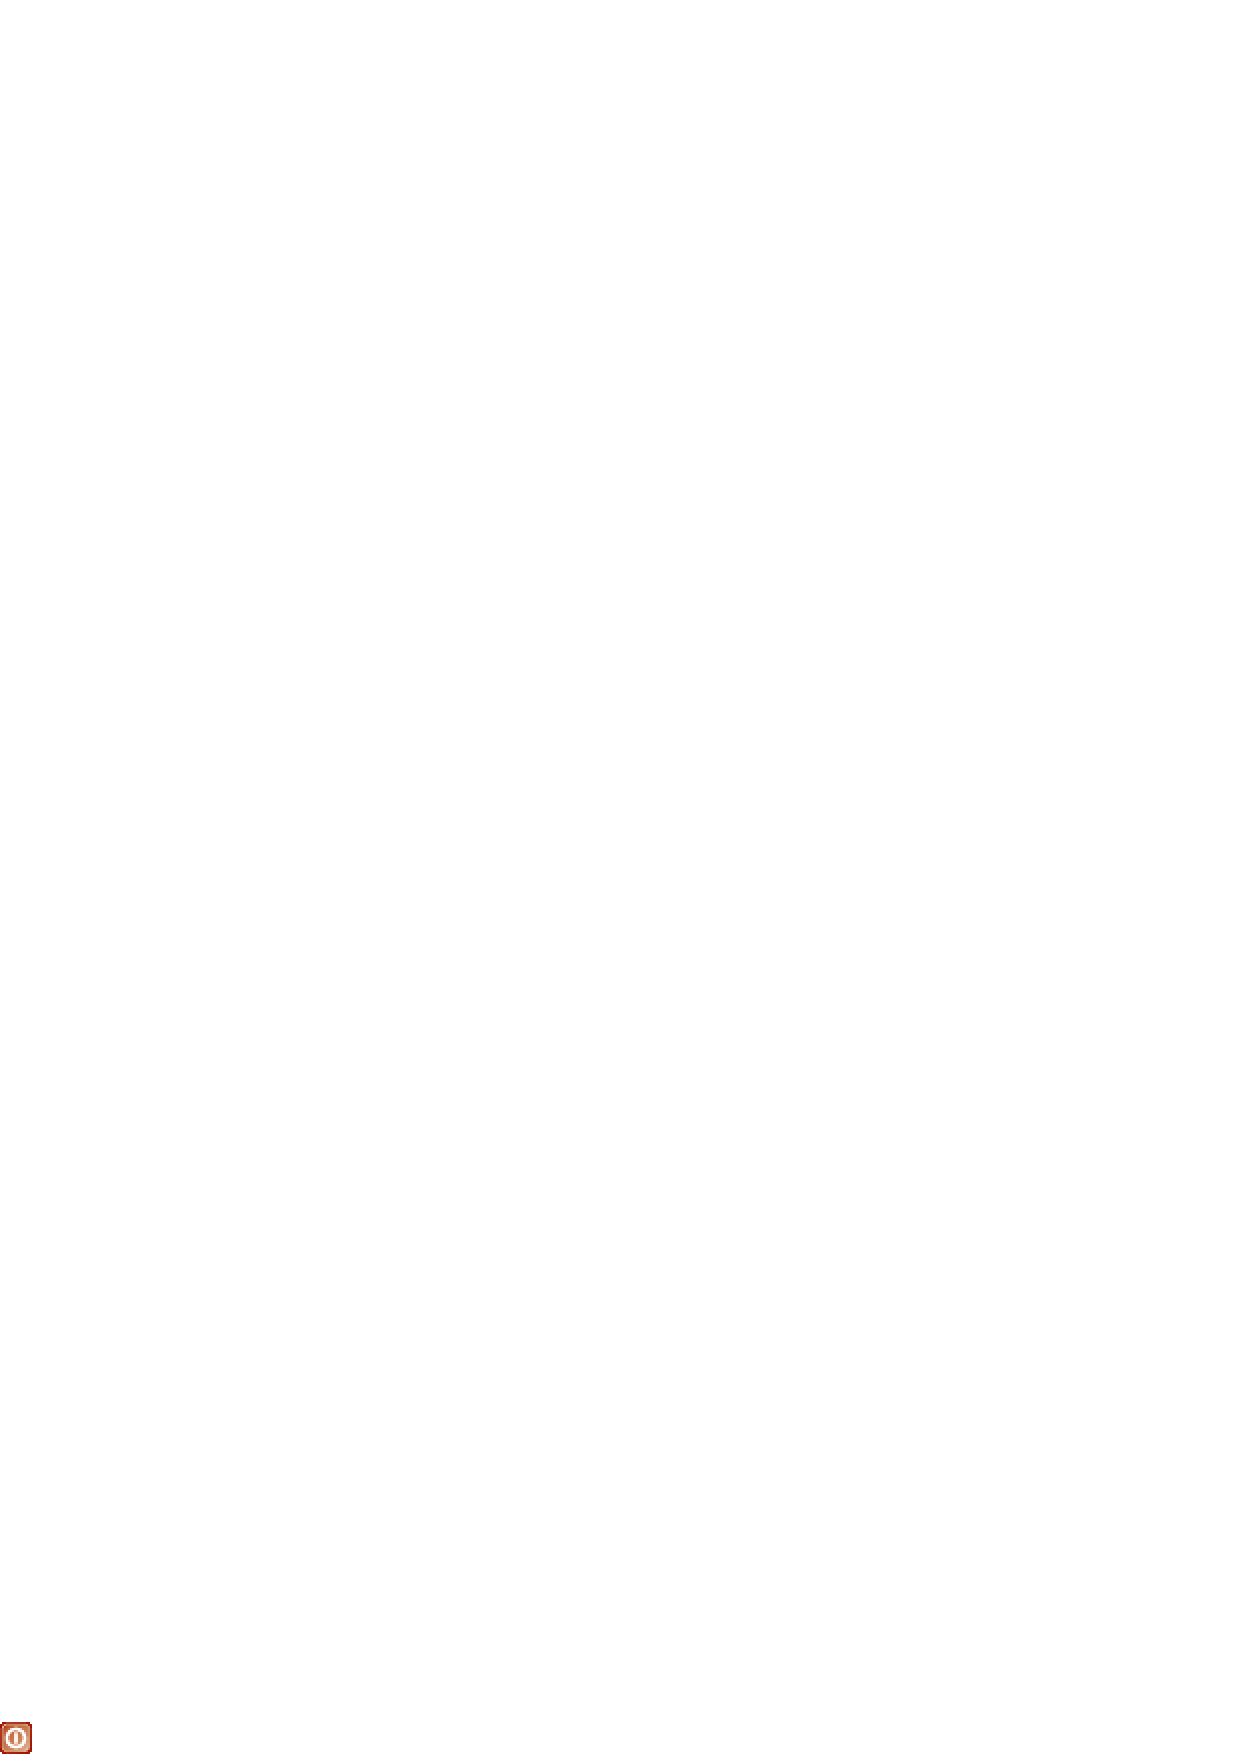
\includegraphics[width=0.7cm]{grass_close_edit} & Cerrar & Cerrar la sesión de digitalización (reconstruye la topología a continuación)\\
\hline
\end{tabular}
\end{table}

\subsubsection{Pestaña Categoría}\index{GRASS!category settings}

Esta pestaña le permite establecer la forma en que se asignará la categoría a cada nuevo objeto espacial y/o asignar una categoría a un objeto espacial.

\begin{itemize}
\item Modo: qué categoría se debería adjuntar a la geometría.
\begin{itemize}
\item La siguiente sin usar: la siguiente categoría que aún no está usada en el archivo vectorial.
\item Entrada manual: definir la categoría en el campo de entrada «Categoría».
\item Ninguna categoría: digitalizar la geometría sin introducir ninguna categoría.
\end{itemize}
\item Categoría: un número (ID) que se adjunta al objeto espacial digitalizado.
\item Capa: identificación del objeto espacial (tabla de atributos).
\end{itemize}

\begin{Tip}\caption{\textsc{Crear «capas» adicionales con QGIS}}
\qgistip{Si quiere añadir más capas a su conjunto de datos, simplemente añada un nuevo número en la casilla «Capa» y pulse Intro. En la pestaña Tabla puede crear una nueva tabla conectada a su nueva capa.
}
\end{Tip}

\subsubsection{Pestaña configuración}\label{label_settingtab}\index{GRASS!snapping tolerance}

Esta pestaña le permite establecer el autoensamblado en píxeles de la pantalla. Esto es el umbral en píxeles en el que los nuevos puntos o finales de líneas son ensamblados de forma automática a nodos existentes. Esto ayuda a evitar saltos o balanceos entre contornos. El valor predeterminado es 10 píxeles.

\subsubsection{Pestaña simbología}\index{GRASS!symbology settings}

Esta pestaña le permite ver y establecer la simbología y la configuración del color para varios tipos de geometría y su estado topológico (ej.: contorno cerrado / abierto).

\subsubsection{Pestaña tabla} \index{GRASS!table editing}
Esta pestaña proporciona información sobre la tabla de la base de datos de una «capa» dada. Aquí puede añadir, modificar o crear nuevas tablas de base de datos para la capa actual.

\begin{Tip}\caption{\textsc{Permisos de edición de GRASS}}\index{GRASS!edit
permissions}
\qgistip{Tiene que ser el propietario del directorio de mapas de GRASS que quiera editar. Es imposible editar vectoriales en directorios de mapas que no sean suyos, incluso si tiene permiso de escritura.
}
\end{Tip} 

\subsection{Herramienta Región}\index{GRASS!region}

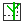
\includegraphics[width=0.7cm]{grass_region_edit} La región actual (ventana) en GRASS es muy importante para todos los módulos ráster. Todos los ráster de nueva creación tienen la extensión y resolución de la región actual, no importa cuál sea su región original. La región se guarda en el archivo \$LOCATION/\$MAPSET/WIND, y define el Norte, Sur, Este, Oeste, número de columnas y filas y la resolución espacial horizontal y vertical.

Es posible encender/apagar la región de GRASS en la vista del mapa de QGIS usando el botón \textsl{Mostrar región actual de GRASS}. \index{GRASS!region!display}

Con el botón \textsl{Editar la región actual de GRASS} puede abrir una herramienta en la que puede cambiar la región actual y la simbología del rectángulo de la región de GRASS en la vista del mapa de QGIS. Cuando se está ejecutando la herramienta también es posible seleccionar una nueva región de forma interactiva con el ratón sobre el lienzo de QGIS.\index{GRASS!region!editing}

% Ambas herramientas sólo están disponibles si QGIS tiene el complemento de GRASS activado.
% was started from a GRASS 
% shell or if the GISRC environment variable pointing to a
% valid GISRC file was set (i.e. only if you are running 
% GRASS within your mapset).

\subsection{Caja de herramientas de GRASS}\index{GRASS!toolbox}

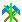
\includegraphics[width=0.7cm]{grass_tools} La caja de herramientas de GRASS proporciona funciones analíticas de GRASS dentro de QGIS. Para usar la caja de herramientas de GRASS necesita tener abierto un directorio de mapas en el que tenga permiso de escritura. Esto es necesario porque QGIS con toda probabilidad creará nuevos conjuntos de datos que necesitarán escribirse en un directorio de mapas válido.

Por lo tanto necesita iniciar QGIS desde dentro de una sesión de GRASS. Así su  directorio de mapas actual se abrirá para escritura.

Otra opción para abrir un directorio de mapas para escritura la proporciona la entrada del complemento de GRASS. Use Complementos->GRASS->Abrir directorio de mapas.

Si tiene el botón de la caja de herramientas de GRASS atenuado, asegúrese de que abrió un directorio de mapas válido para escritura, puesto que el complemento de GRASS necesita un directorio de mapas para guardar sus resultados.

La caja de herramientas también proporciona un explorador de datos muy útil para nevegar por su localización actual y los directorios de mapas que contiene.


\subsubsection{Módulos dentro de la caja de herramientas} \index{GRASS!toolbox!modules}

La caja de herramientas de GRASS proporciona una colección de móculos de GRASS que se pueden usar desde dentro de QGIS. Están agrupados en bloques temáticos que se pueden definir por el usuario (vea la Sección \ref{sec:toolbox-customizing}).

Cuando pulse en un módulo se añadirá una nueva pestaña a su caja de herramientas que proporciona tres nuevas subpestañas:
\begin{enumerate}
\item Opciones
\item Salida 
\item Manual
\end{enumerate}

\minisec{Opciones}

Esta pestaña proporciona un campo de entrada muy simplificado en el que tiene que seleccionar los mapas necesarios e introducir los parámetros para ejecutar el módulo seleccionado. Tenga en cuenta que estas opciones se mantienen lo más simples posible, con el fin de mantener clara la estructura. Si necesita más opciones del módulo, siéntase libre de usar la consola de GRASS para ejecutar el módulo.

\minisec{Salida}

Esta pestaña proporciona la salida generada por el módulo que se está ejecutando. Después de pulsar el botón «Ejecutar», el módulo pasa a la pestaña Salida y verá información sobre el proceso. Si todo va bien, verá \texttt{Finalizado correctamente} al final.

\minisec{Manual}

Esta pestaña muesta la página de ayuda de cada módulo de GRASS. Puede echar un vistazo a la página del manual si quiere tener un conocimiento mayor sobre el objetivo del módulo. Puede que se haya dado cuenta de que algunos módulos tienen más opciones y parámetros que los que aparecen en la pestaña \textit{Opciones}. Esto es correcto y hecho así por diseño. Para mantener la interfaz de usuario lo más simple posible, sólo se ponen las opciones y parámetros necesarios en la pestaña Opciones. Pero siempre puede usar la consola de GRASS para ejecutar el módulo con todos sus parámetros.

\begin{Tip}\caption{\textsc{Mostrar resultados inmediatamente}}\index{GRASS!display results}
\qgistip{Si quiere mostrar los resultados de sus cálculos inmediatamente en el lienzo de su mapa, puede usar el botón «Ver salida» de la parte inferior de la pestaña del módulo.
}
\end{Tip} 


\subsubsection{Explorador de GRASS} \index{GRASS!toolbox!Browser}

Otra función útil es el explorador de GRASS. En la Figura~\ref{subfig:grass_browser} puede ver la localización actual con su directorio de mapas.

El explorador de la izquierda la permite navegar por todos sus directorios de mapas dentro de la localización seleccionada.

La parte derecha de la ventana del explorador muestra alguna metainformación del conjunto de datos seleccionado, por ejemplo la resolución, límites exteriores, fuente de datos, tabla de atributos para datos vectoriales\dots

La barra de herramientas que hay dentro de la pestaña Explorador la proporciona las siguientes herramientas para el conjunto de datos seleccionado:
\begin{itemize}
\item 
\includegraphics[width=0.7cm]{grass_add_map} Añadir el mapa seleccionado a la vista del mapa.
\item 
\includegraphics[width=0.7cm]{grass_copy_map} Copiar el mapa seleccionado.
\item 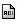
\includegraphics[width=0.7cm]{grass_rename_map} Cambiar el nombre al mapa seleccionado.
\item 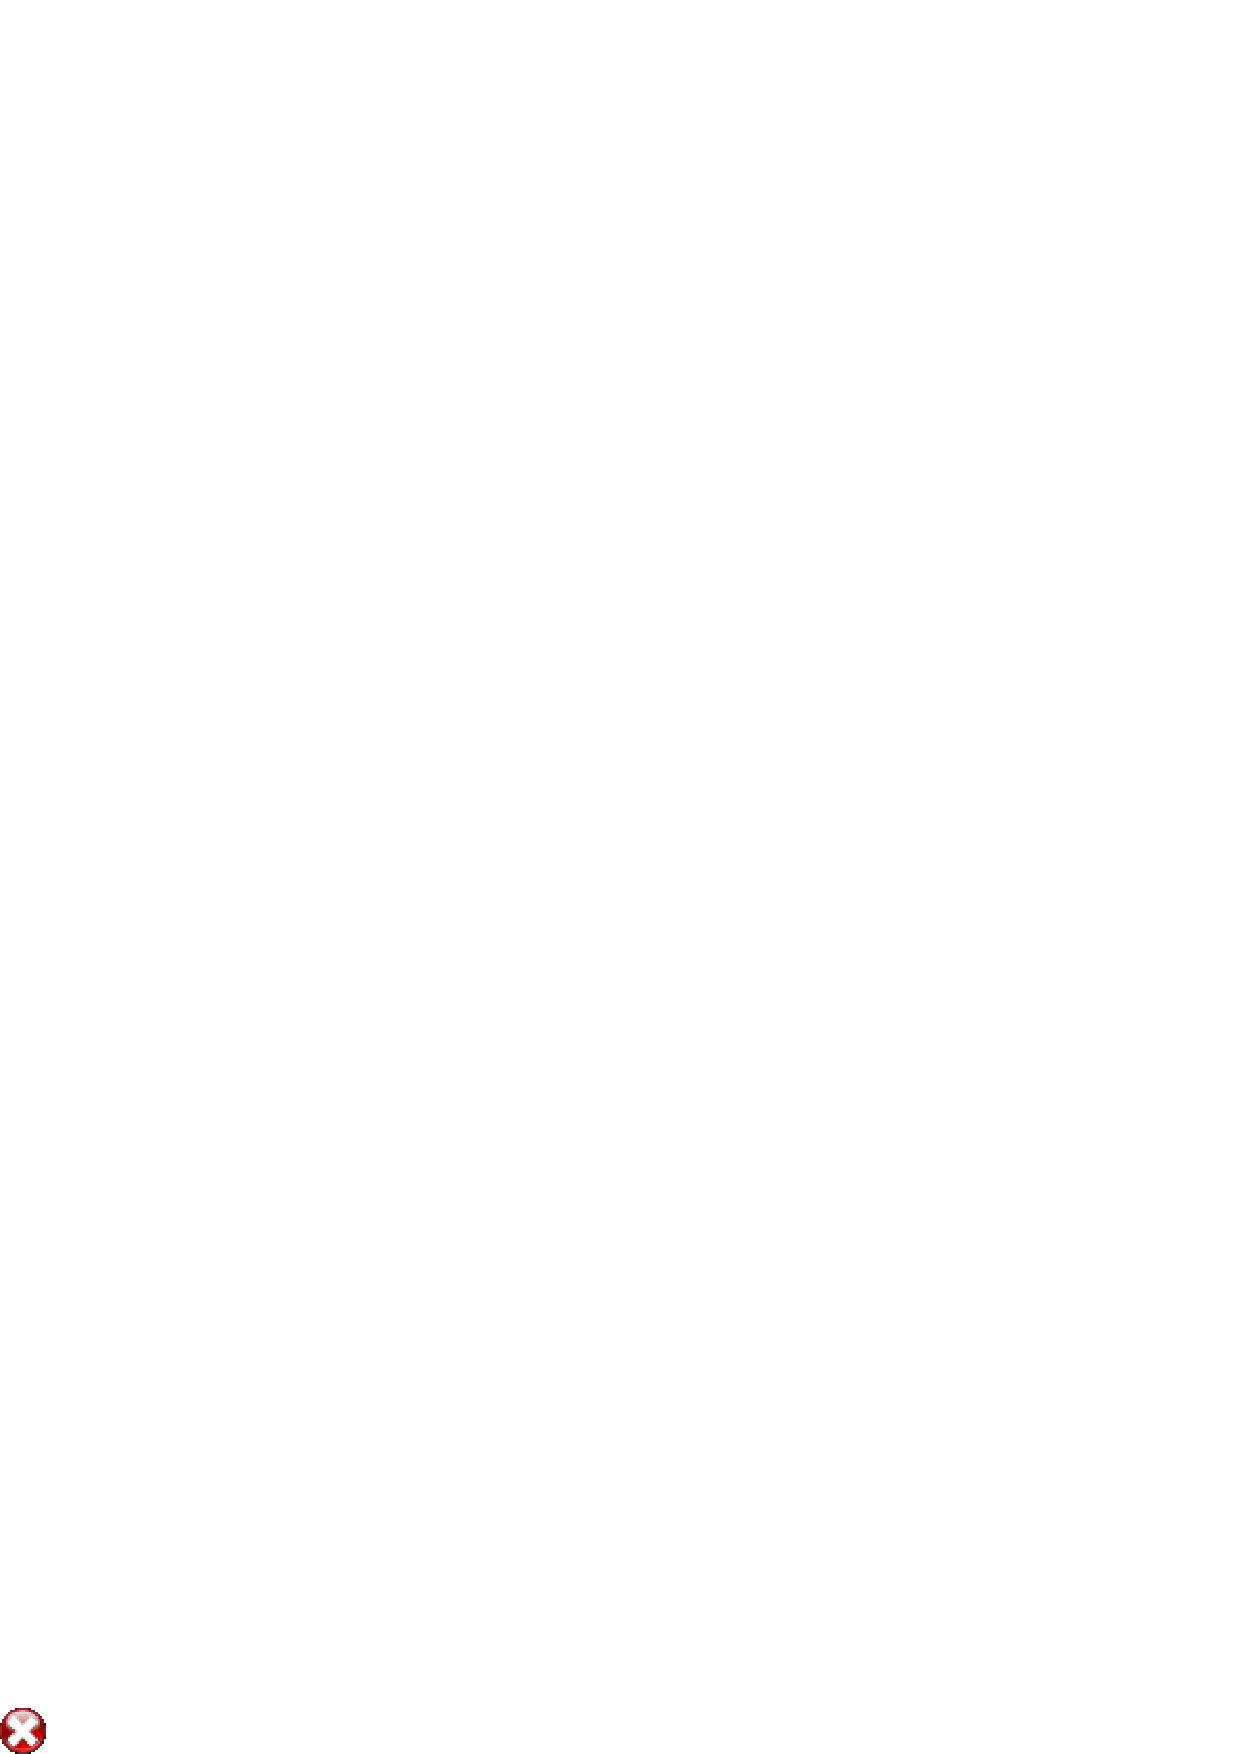
\includegraphics[width=0.7cm]{grass_delete_map} Borrar el mapa seleccionado.
\item 
\includegraphics[width=0.7cm]{grass_set_region} Establecer la región actual al mapa seleccionado.
\item 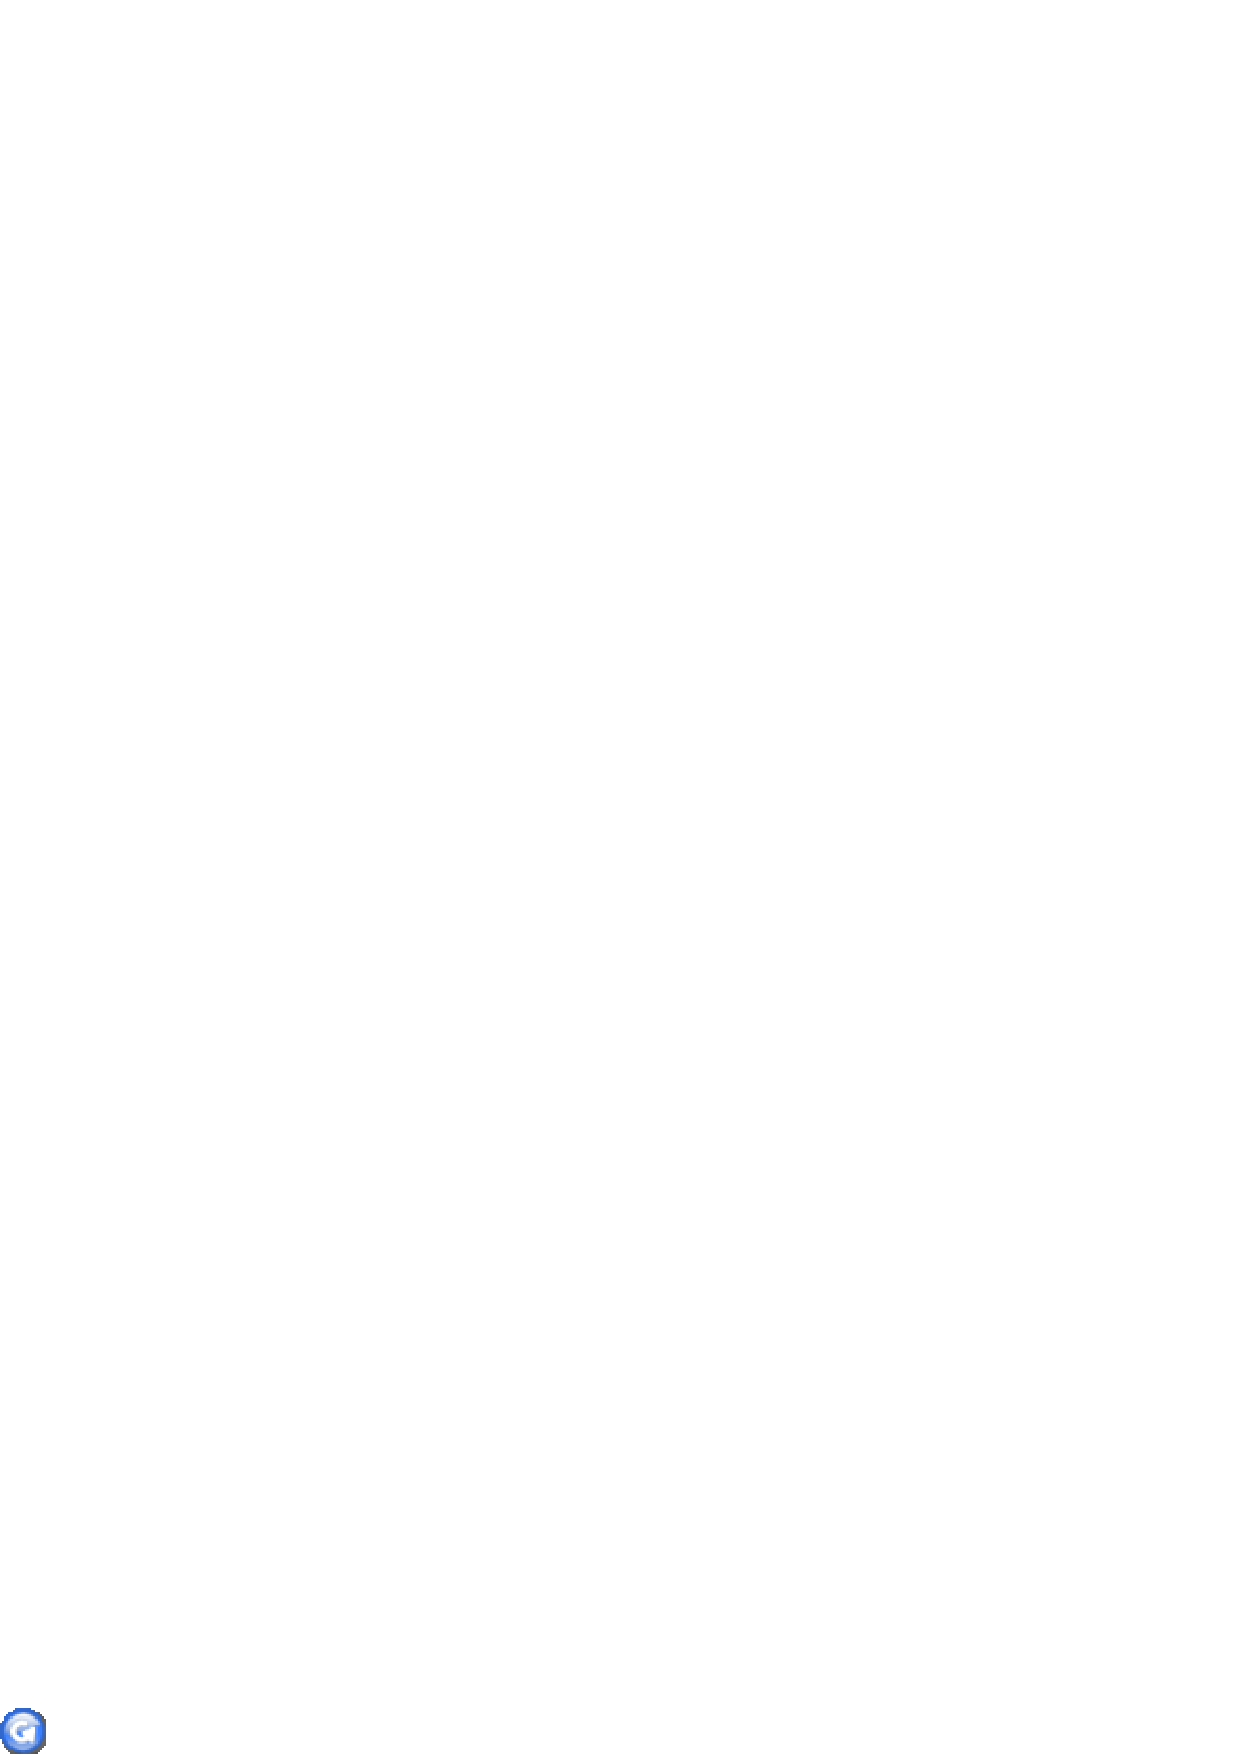
\includegraphics[width=0.7cm]{grass_refresh} Actualizar la ventana del explorador.
\end{itemize}

Los botones «Cambiar nombre» y «Borrar» sólo están disponibles en su directorio de mapas actual. Todas las demás herramientas también funcionan en mapas de otros directorios de mapas.

% Picture from the GRASS-Browser here:
\begin{figure}[h]
\centering
	\caption{Caja de herramientas de GRASS}
   \subfigure[Explorador de GRASS dentro de la caja de herramientas]{\label{subfig:grass_browser}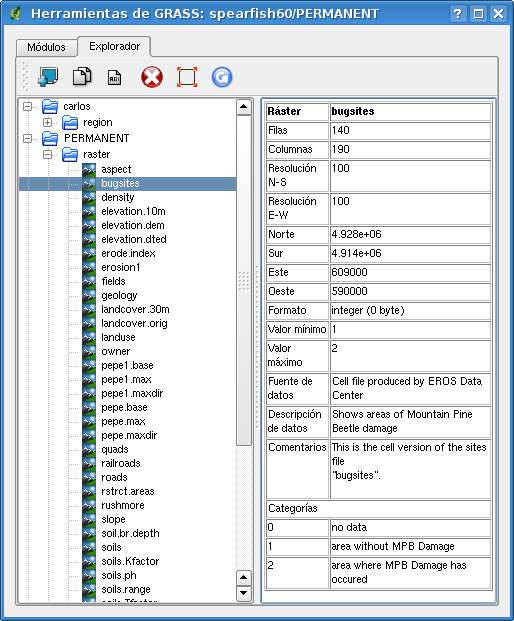
\includegraphics[clip=true, width=0.4\textwidth]{grassbrowser}}\goodgap
   \subfigure[Consola de GRASS dentro de la caja de herramientas]{\label{subfig:grass_shell}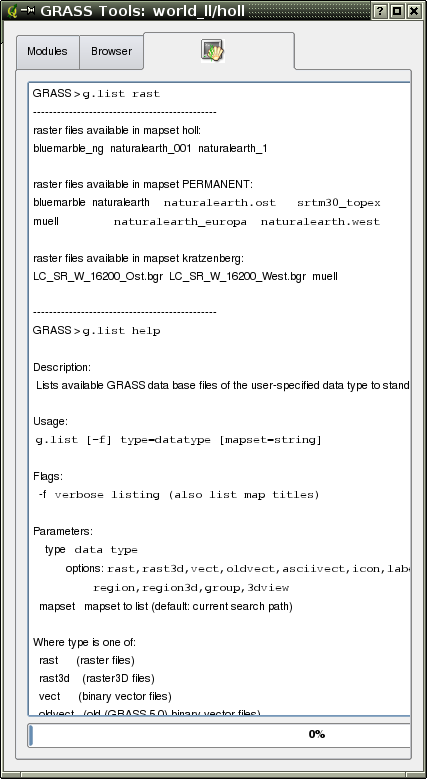
\includegraphics[clip=true, width=0.4\textwidth]{grassshell}}
\end{figure}

\subsubsection{Personalizar la sección de los módulos} \index{GRASS!toolbox!customize}
\label{sec:toolbox-customizing}

Casi todos los módulos de GRASS se pueden añadir a la caja de herramientas de GRASS. Se proporciona una interfaz XML para analizar los sencillos archivos XML que configuran los módulos dentro de la caja de herramientas.

% TODO: migrating the content of this wiki-page into the manual?
Se puede encontrar una breve descripción sobre cómo añadir nuevos módulos, cambiar los grupos de módulos, etc. en el wiki de QGIS en \url{http://wiki.qgis.org/qgiswiki/Adding\_New\_Tools\_to\_the\_GRASS\_Toolbox}.

Un ejemplo de archivo XML para generar el módulo \texttt{v.buffer} (v.buffer.qgm) tiene este aspecto:
\begin{verbatim}
<?xml version="1.0" encoding="UTF-8"?>
<!DOCTYPE qgisgrassmodule SYSTEM "http://mrcc.com/qgisgrassmodule.dtd">

<qgisgrassmodule label="Vector buffer" module="v.buffer">
        <option key="input" typeoption="type" layeroption="layer" />
        <option key="buffer"/>
        <option key="output" />
</qgisgrassmodule>
\end{verbatim}

\begin{figure}[ht]
\centering
\caption{Módulo generado mediente el análisis del archivo XML}\label{fig:buffer-module}
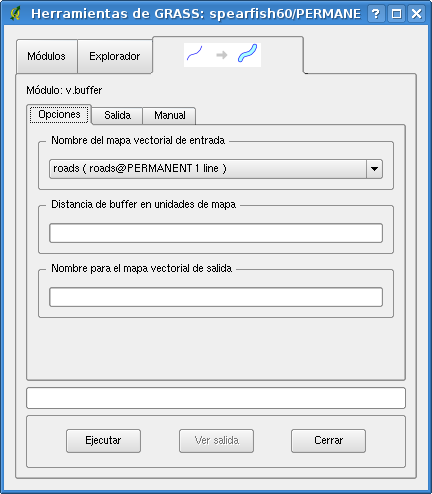
\includegraphics[clip=true, width=0.45\textwidth]{vbuffer}
\end{figure}

El analizador lee esta definición y crea una pestaña nueva dentro de la caja de herramientas cuando selecciona el módulo:


\subsection{Crear una nueva capa de GRASS}\label{sec:creating_new_grass_vectors}\index{GRASS!Creating new vectors|see{editing!creating a new layer}}

Con esta versión de QGIS también es posible crear nuevos vectoriales desde dentro de GRASS muy fácilmente.

Simplemente seleccione \textsl{Complementos->GRASS->Crear nuevo vectorial de GRASS} de la barra de herramientas, dele un nombre nuevo en el cuadro de texto y comience a digitalizar. Si encuentra el botón atenuado, asegúrese de que tiene activado un directorio de mapas de trabajo. Si olvidó cómo activar un directorio de mapas eche un vistazo a la Sección \ref{sec:load_grassdata}.

Puesto que GRASS es capaz de organizar todo tipo de geometrías en una capa, no hay necesidad de seleccionar la geometría. Ésto sólo se aplica a la creación de archivos shape (vea la sección \ref{sec:create shape}).

Algunos consejos para hacer su digitalización más útil:
\begin{itemize}
\item Asegúrese de crear una tabla de atributos con las columnas necesarias antes de empezar a digitalizar si quiere asignar atributos a sus objetos digitalizados. Vaya a la pestaña Tabla dentro de la ventana de digitalización.
\item Si planea crear una capa de polígonos, considere establecer el modo a \textsl{Sin categoría}. A continuación empiece a digitalizar los contornos que realmente no necesitan una entrada en la tabla de atributos. Si ha hecho esto, vuelva a cambiar a \textsl{La siguiente sin usar} y comience a digitalizar los centroides, que contienen la información de los atributos de un polígono.

\end{itemize}

%\section{The GRASS Toolbar}
%The GRASS toolbar is displayed when the GRASS plugin is loaded using the
% Plugin Manager (see Section \ref{sec:managing_plugins}, \textsl{Managing
% Plugins}). Figure  shows the toolbar with each function annotated.